\documentclass{article}
\usepackage{tikz}
\usepackage{music}
\usetikzlibrary{calc,positioning}

\begin{document}

% Example: Bezier curve for gamaka between notes
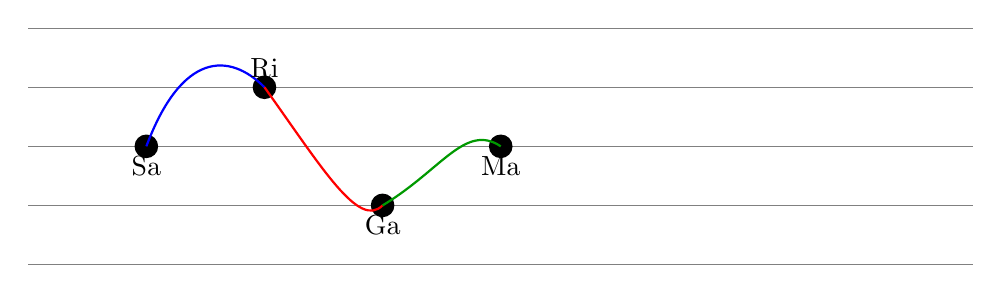
\begin{tikzpicture}[scale=1.5]
    % Staff lines
    \foreach \y in {0,0.5,1,1.5,2} {
        \draw[gray,thin] (0,\y) -- (8,\y);
    }
    
    % Notes positions
    \coordinate (n1) at (1,1);    % Sa
    \coordinate (n2) at (2,1.5);  % Ri
    \coordinate (n3) at (3,0.5);  % Ga
    \coordinate (n4) at (4,1);    % Ma
    
    % Draw notes
    \foreach \n in {n1,n2,n3,n4} {
        \fill (\n) circle (0.1);
    }
    
    % Gamaka curves (Bezier)
    \draw[thick,blue] (n1) .. controls (1.3,1.8) and (1.7,1.8) .. (n2);
    \draw[thick,red] (n2) .. controls (2.5,0.8) and (2.8,0.3) .. (n3);
    \draw[thick,green!60!black] (n3) .. controls (3.5,0.8) and (3.7,1.2) .. (n4);
    
    % Labels
    \node[below] at (n1) {Sa};
    \node[above] at (n2) {Ri};
    \node[below] at (n3) {Ga};
    \node[below] at (n4) {Ma};
\end{tikzpicture}

\vspace{1cm}

% More complex gamaka pattern
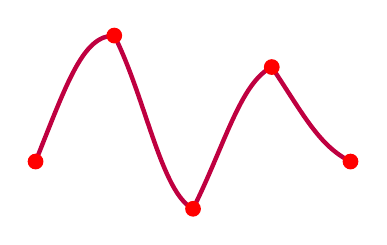
\begin{tikzpicture}[scale=2]
    % Define control points for complex gamaka
    \coordinate (start) at (0,0);
    \coordinate (peak1) at (0.5,0.8);
    \coordinate (valley) at (1,-0.3);
    \coordinate (peak2) at (1.5,0.6);
    \coordinate (end) at (2,0);
    
    % Draw the gamaka curve
    \draw[ultra thick,purple] 
        (start) .. controls (0.2,0.5) and (0.3,0.8) .. (peak1)
                .. controls (0.7,0.4) and (0.8,-0.2) .. (valley)
                .. controls (1.2,0.1) and (1.3,0.5) .. (peak2)
                .. controls (1.7,0.3) and (1.8,0.1) .. (end);
    
    % Mark key points
    \foreach \p in {start,peak1,valley,peak2,end} {
        \fill[red] (\p) circle (0.05);
    }
\end{tikzpicture}

\end{document}